\chapter{Measurement of Weak Lensing and the Cosmic Microwave Background}
\section{Weak Lensing}
In general, contemporary weak lensing surveys measure the light emmited from galaxies in two components: galaxy position and galaxy shear. In the following sections the theoretical base for cosmological weak lensing surveys are described. However, before discussing the two relevant observables, one needs to formalize the concept of weak lensing.
\begin{figure}[ht]
	\centering
	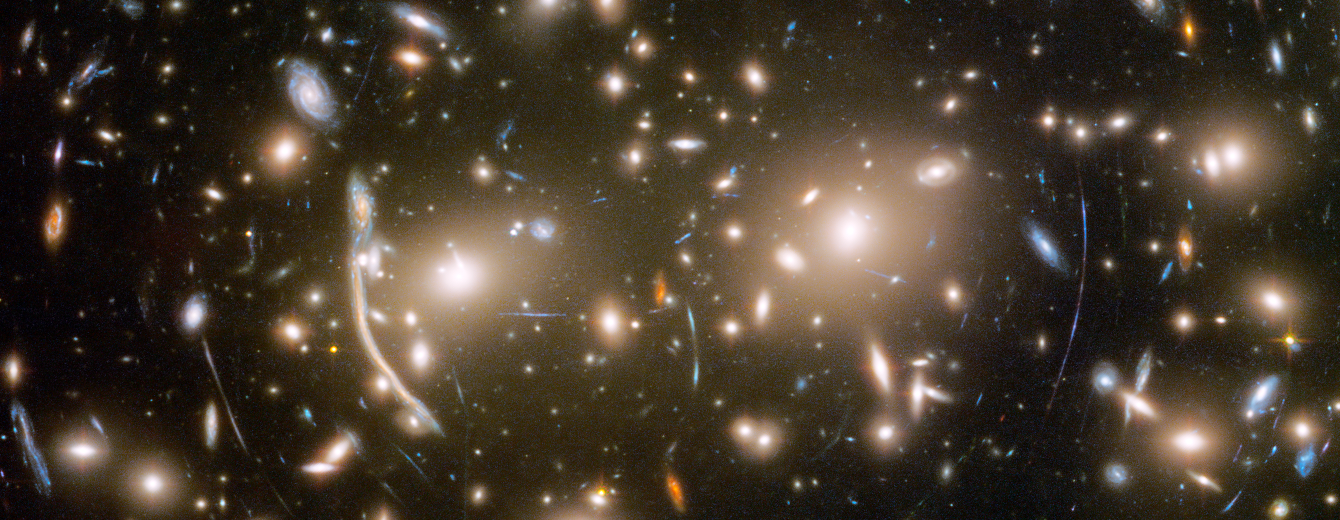
\includegraphics[width=\textwidth]{plots/hubble_weak_lensing.png}
	\caption{Image of weak lensing taken by the Hubble Space Telescope~\cite{hubble_lensing}.}
	\label{fig:weak_lensing}
\end{figure}
\subsection{The Linear Matter Power Spectrum}
As we have seen before, we consider deviations from the FLRW metric using the scalar fields $\Phi$ and $\Psi$. In the absence of anisotropic stress, $\Phi=-\Psi$, which we will assume here for demonstration (one can use codes such as CAMB or CLASS to do computations including anisotropy if desired). 

Throughout time in the universe, we consider there to be three distinct epochs/regions~\cite{scott_dodelson_modern_2021}:
\begin{itemize}
	\item The super-horizon region, or the region before inflation where radiation dominates
	\item The horizon-crossing region, or the region during inflation where the universe transfers from radiation to matter domination
	\item The sub-horizon region, or the region of after rapid inflation where matter dominates
\end{itemize}
Additionally, the formation of matter inhomogeneity comes from gravitational instability, the idea that primordial curvature perturbations in the super-horizon grew to form small matter density contrasts which grew in size after crossing the horizon. After the rate of inflation slowed, gravitational forces caused clusters of matter to become the galaxies and clusters we see today.

This gives us a blueprint for writing the matter power spectrum. We have the primordial curvature perturbation $\mathcal{R}$ which source the inital matter inhomogeneity that formed late-time large scale structure. Thus, we can write it as
\begin{equation}
	\mathcal{R} = \frac{5}{3}\Phi_{\text{large-scale}}(k,a_{\text{late}})
\end{equation} 
Additionally, we have a transfer function which describes the transition from radiation to matter domination, defined as
\begin{equation}
	T(k) = \frac{\Phi(k,a_{\text{late}})}{\Phi_{\text{large-scale}(k,a_{\text{late}})}}
\end{equation}
And we have a growth factor, defined as the linear growth of matter density contrast during matter domination, defined as
\begin{equation}
	D_+(a) = a \frac{\Phi(k,a)}{\Phi(k,a_{\text{late}})}
\end{equation}
Thus we can write the gravitational potential at all times as
\begin{equation}
	\Phi(k,a) = \frac{3}{5a}\mathcal{R}(k)T(k,a)D_+(a)
\end{equation}
This together with the Poisson equation for the matter density contrast field gives the equation
\begin{equation}
	\delta_m(k) = \frac{2k^2a}{3\Omega_mH_0^2}\Phi(k,a)
\end{equation}
\begin{equation}
	\delta_m(k) = \frac{2}{5}\frac{k^2}{\Omega_mH_0^2}\mathcal{R}(k)T(k,a)D_+(a)
\end{equation}
The power spectrum of an observable is defined as the two-point correlation function of the observable in Fourier space.
\begin{equation}
	P_\mathcal{O}(k) = \langle \mathcal{O}(k)\mathcal{O}(k) \rangle
\end{equation}
Thus the linear matter power spectrum (because we restricted the matter density contrast field to linear order terms in the perturbation) is given by
\begin{equation}
	\begin{split}
		P_m^{L}(k,a) = \frac{8\pi^2}{25 \Omega_m^2 H_0^4} A_s D_+^2(a)T^2(k)\frac{k^{n_s}}{k_p^{(n_s-1)}}
	\end{split}
\end{equation}

\subsection{Galaxy Density}
In practice, we cannot measure the matter power spectrum. Dark matter prohibits direct measurement, thus one must determine observables which trace the matter distribution in the universe. The most natural option is to observe the galaxy distribution. However, large scale structures and galaxies provide many sources for non-linearities in the power spectrum and result in a non-trivial relation between the two. By taking certain data selection criteria, one can cut out the non-linear contributions. The relation between the galaxy and matter power spectra are then related by the linear bias factor.
\begin{equation}
	\begin{split}
		\delta_g(k) &= b_1 \delta_m(k) \\
		P_g(k,a) &= (b_1)^2P_m^L(k,a)
	\end{split}
\end{equation}
Realistically, in galaxy surveys we do not have access to exact reshifts for each observed galaxy. Rather, an image is taken of the sky in multiple color bands from which the redshift is determined. This procedure is called photometric redshift. To account for this, one can attempt to redefine the galaxy power spectrum. First, we define the distribution of distances as
\begin{equation}
	W(\chi) = \frac{1}{N_g}\frac{dN_g}{d\chi}
\end{equation}
The procedure for determining this distribution will be discussed in section (section for dz and IA). This allows us to simply write the projected density contrast as
\begin{equation}
	\Delta_g = \int\limits_0^\infty W(\chi)\delta_g(x,\tau)d\chi
\end{equation}
To complete this discussion, we will make some approximations. We will only consider small scales for which $\sin(\theta)\sim \theta \sim 1/l$ where $l$ is the Fourier conjugate of $\theta$. Second is the limber approximation, which states that, as long as the galaxy power spectrum $P_g$ slowly varies over the region $\Delta k \sim 1/l\chi$, we approximate is as a constant. These approximations greatly simplify the integrals required when computing power spectrum of Fourier transformed $\Delta_g$. This power spectrum is called the angular power spectrum. Taking into account the approximations above and computing the fourier transfrom, one finds an angular power spectrum of
\begin{equation}
 	C_g(l) =\int \frac{1}{\chi^2}W^2(\chi)P_g(k=(l+1/2)/\chi,\eta) d\chi
\end{equation} 
\subsection{Galaxy Shear}
Photons move on null geodesics, thus $d\chi = -d\eta$, where $\eta$ is the conformal time and $\chi$ is the conformal distance. This tells us that $dx^i/d\chi = -dx^i/d\eta = -a dx^i/dt = -a dx^i/d\lambda d\lambda/dt = -a/P^0 P^\mu = -a / E * p/a \hat{p}^i = -\hat{p}^i$ (for photons and other massless particles).
Thus, under lensing, the difference between the observed and true positions within the source plane is given by
\begin{equation}
	\chi\mathbf{\theta}^i = x_\perp^i = -\int\limits_0^\chi \hat{p}^i_\perp(\chi'') d\chi''
\end{equation}
Our goal is to write this as a function of the potential only. Thus we look to compute $d\hat{p}^i/dt$.
\begin{equation}
	\begin{split}
		\frac{d\hat{p}^i}{dt} %=& \frac{d}{dt}\frac{1}{p}p^i \\
		=& \frac{1}{p^2}(\dot{p}^i p - \dot{p}p^i)
	\end{split}
\end{equation}
By computing $\dot p^i$, we can find $\dot p$ as well.
\begin{equation}
	\begin{split}
		\frac{dp^i}{d\lambda} %=& \frac{d}{d\lambda}\left(aP^i(1+\Phi)\right) \\
		=& P^i\frac{d}{d\lambda}(a(1+\Phi)+(1+\Phi)a\frac{d}{d\lambda}P^i
	\end{split}
\end{equation}
We have $d/d\lambda = P^\mu \partial_\mu$, so the first term becomes
\begin{equation}
	\begin{split}
		P^i\frac{d}{d\lambda}(a(1+\Phi)) %&= P^iP^\mu \partial_\mu(a(1+\Phi)) \\
		%&= P^iP^0(\dot a + a\dot\Phi + \dot a \Phi) + a P^iP^j \partial_j\Phi \\
		&= a P^i (P^0(H+\dot\Phi +H\Phi) + P^j\partial_j\Phi) \\
	\end{split}
\end{equation}
The second term is evaluated by using the geodesic equation up to first order in the perturbations.
\begin{equation}
	\begin{split}
		\frac{d}{d\lambda}P^i &= -\Gamma^i_{\mu\nu}P^\mu P^\nu \\
		%&= -(P^0)^2\frac{1}{a^2}\partial^i\Psi - 2\delta^{i}_{j}(H+\dot\Phi)P^0P^j + 2P^iP^j\partial_j\Phi - P^jP_j\partial^i\Phi \\
		%&= -E(1-\Psi)\left( \frac{E}{a^2} \partial^i\Psi + \frac{1}{a}2p^i(1-\Phi)(H+\dot\Phi) - \frac{2}{a^2E}p^ip^j\partial_j\Phi + \frac{p^2}{a^2E} \partial^i\Phi \right) \\
		&= -E\left( \frac{E}{a^2} \partial^i\Psi + \frac{1}{a}2p^i(1-\Phi-\Psi)(H+\dot\Phi) - \frac{2}{a^2E}p^ip^j\partial_j\Phi + \frac{p^2}{a^2E} \partial^i\Phi \right)
	\end{split}
\end{equation}
Plugging everything back in, and only keeping terms to linear order, we get
\begin{equation}
	\begin{split}
		%=& aP^i(H+\dot\Phi+H\Phi) + aP^iP^j\partial_j\Phi \\
		%& - \frac{E}{a}\partial^i\Psi - 2p^i(H+\dot\Phi) + \frac{2}{aE}p^ip^j \partial_j\Phi - \frac{p^2}{aE}\partial^i\Phi \\
		\frac{dp^i}{dt} %=& p^i(1-\Phi)(H+\dot\Phi+H\Phi) + (1-\Phi)^2p^ip^j\partial_j\Phi \\
		%& - \frac{E}{a^2}\partial^i\Psi -\frac{2p^i}{a}(H+\dot\Phi) + \frac{2}{a^2E}p^ip^j \partial_j\Phi - \frac{p^2}{a^2E}\partial^i\Phi \\
		%=& p^i(H+\dot\Phi) + \frac{p^ip^j}{aE}\partial_j\Phi \\
		%& - \frac{E}{a}\partial^i\Psi -2p^i(H+\dot\Phi) + \frac{2}{aE}p^ip^j \partial_j\Phi - \frac{p^2}{aE}\partial^i\Phi \\
		=& -p^i(H+\dot\Phi)- \frac{1}{aE}\left(p^ip^j\partial_j\Phi - p^2\partial^i\Phi\right) -\frac{E}{a}\partial^i\Psi
	\end{split}
\end{equation}
The time derivative of the modulus of the momentum, $p$, is then given by
\begin{equation}
	\begin{split}
		\frac{dp}{dt} =& \frac{d}{dt}\sqrt{\delta_{ij}p^ip^j} = \frac{1}{p}\delta_{ij}\dot p^i p^j \\
		%=& -p(H+\dot\Phi) - \frac{p}{aE}(p^i\partial_i\Phi - pp^i\partial^i\Phi) - p^i\frac{E}{ap}\partial^i\Psi \\
		=& -p(H+\dot\Phi) - \hat{p}_i\frac{E}{a}\partial^i\Psi
	\end{split}
\end{equation}
Now, putting everything together, plugging these results into eq () gives
\begin{equation}
	\begin{split}
		\frac{d\hat{p}^i}{dt} %=& -\hat{p}^i(H+\dot\Phi)- \frac{1}{aEp}\left(p^ip^j\partial_j\Phi - p\partial^i\Phi\right) -\frac{E}{ap}\partial^i\Psi + \hat{p}^i\left( (H+\dot\Phi) + \hat{p}_i\frac{E}{ap^2}\partial^i\Psi \right) \\
		=&  \frac{E}{ap}\left( \frac{p^2}{E^2}\partial_j\Phi - \partial_j\Psi \right)(\delta^{ij}-\hat{p}^i\hat{p}^j)
	\end{split}
\end{equation} 
Going back to the photon scenario, where $E=p$, this simplifies to
\begin{equation}
	\frac{d\hat{p}^i}{dt} = \frac{1}{a}\left( \partial_j\Phi - \partial_j\Psi \right)(\delta^{ij}-\hat{p}^i\hat{p}^j)
\end{equation}
Interestingly, $\delta^{ij}-\hat p^i \hat p^j$, is the projection operator of the $j$-th direction onto the $i$-th. So, if we orient our axes so that the photon approximately travels along the $j$-th direction, we can sum of $i$ and $k$ so that the orthogonal components of the momentum are evaluated by
\begin{equation}
	\frac{d\hat{p}^i_\perp}{d\chi} = - a \frac{d\hat{p}^i_\perp}{dt} = -\partial_i(\Phi-\Psi)
\end{equation}
In the absence of anisotropic stress (like in the late universe where weak lensing is measured), $\Phi=-\Psi$ and 
\begin{equation}
	\frac{d\hat{p}^i_\perp}{d\chi} -2\partial_i\Phi
\end{equation}
Integrating this equation gives us
\begin{equation}
	\hat p_\perp (\chi'') = -2\int\limits_0^{\chi''}\partial_i\Phi(\chi') d\chi' + C_i
\end{equation}
where the constant $C_i$ comes from integrating a derivative, where it is only defined up to a constant. Now, plugging back in we have
\begin{equation}
	\mathbf{\theta}^i = \frac{2}{\chi}\int\limits_0^\chi \int\limits_0^{\chi''}\partial_i\Phi(\chi') d\chi' d\chi'' - C_i
\end{equation}
In the absence of lensing, this should reduce to $\mathbf{\theta}^i = \theta_0$, the true source position. Hence $C^i=\theta^i_0$ and the total deflection angle is given by
\begin{equation}
	\begin{split}
		\Delta\theta^i =& \frac{2}{\chi}\int\limits_0^\chi \int\limits_0^{\chi''}\partial_i\Phi(\chi') d\chi' d\chi''\\
		=& \frac{2}{\chi}\int\limits_0^\chi \partial_i\Phi(\chi') (\chi-\chi') d\chi'
	\end{split}
\end{equation}
Finally, since $x^i=\chi\theta^i$, we have $\partial_i = \partial_{\theta^i}/\chi$. Now we introduce the \textit{lensing potential} defined by
\begin{equation}
	\begin{split}
		\Delta\theta^i =& \frac{\partial}{\partial \theta^i}\psi_L(\theta) \\
		\psi_L(\theta) =& 2\int\limits_0^\chi \frac{1}{\chi'}\Phi(\chi') \left(1-\frac{\chi'}{\chi}\right) d\chi'
	\end{split}
\end{equation}
This result is great, but it's not very experimentally illuminating. Similar to the galaxy vs matter power spectrum, the absence of the observation of dark matter means we cannot reliably determine the potential $\Phi$. Again, an attempt to relate the lensing potential to some property of galaxies can give us a measureable quantity. Lensing distorts the shape of the galaxies (see figure~\ref{fig:weak_lensing}), where we assume all galaxies are elliptical. Define the galaxy shape tensor by
\begin{equation}
	q_{ij} \equiv \frac{1}{F}\int I\theta^i\theta^j d\theta^i d\theta^j
\end{equation}
This integral is symmetric under $i \leftrightarrow j$. Writing this as a matrix gives
\begin{equation}
	q_{ij} = \frac{1}{2} \text{tr}(q) \left( 
	\begin{array}{cc}
	1+\epsilon_1 & \epsilon_2 \\
	\epsilon_2 & 1-\epsilon_1
	\end{array}
	\right)
\end{equation}
Shape distortion specifically occurs when the deflection angle is not constant across a galaxy. Thus we can look at the tranformation tensor as
\begin{equation}
	A_{ij} \equiv \frac{\partial \theta^i_S}{\partial\theta^j} = \left( 
	\begin{array}{cc}
	1+\kappa - \gamma_+ & -\gamma_\times \\
	-\gamma_\times & 1+\kappa+\gamma_+
	\end{array}
	\right) = \delta_{ij}+\psi_{ij}
\end{equation}
Within this tensor, the $\gamma_+$ and $\gamma_-$ represent shear and $\kappa$ represents magnification and changes in galaxy light flux ($F$). The $E$-mode is given by
\begin{equation}
	E(l) = \left( \frac{l^il^j}{l^2} - \frac{1}{2}\delta^{ij} \right)(-\psi^{ij}(l))
\end{equation}
Which relates to the shear components by
\begin{equation}
	\left(
	\begin{array}{c}
	\gamma_+ \\
	\gamma_\times
	\end{array}
	\right)
	=
	\left(
	\begin{array}{c}
	\cos(2\alpha_l) \\
	\sin(2\alpha_l)
	\end{array}
	\right)
	E(l)
\end{equation}
This connects the observable shear to the theoretical lensing potential.
\subsection{Weak Lensing Correlation Functions}
In the previous two sections, we have derived two observables directly connected to cosmological theories. By observing the galaxies we can determine $\Omega_b$, $A_s$, $n_s$ and $H_0$. By observing shear we can determine $\Omega_m$. The details for how to determine these parameters will be discuss in chapter (chapter). Together these two can fully determine the values of the 5 $\Lambda$CDM parameters. We are still not ready, since these two quantities themselves are not observables. Using these two quantities, however, one can construct three different two-point correlation functions which are observable.

The first correlation function is the autocorrelation of galaxy density, called galaxy clustering. Given a density in a particular angular position, the correlation function can be interpreted as the likelihood of observing a similar density at another close position. The galaxy clustering correlation function is given by
\begin{equation}
	w_g(\theta) = \mathcal{F}(C_g(l)) = \frac{1}{2\pi}\int\limits_0^\infty l C_g(l) J_0(l\theta)dl
\end{equation}
Where $J_0$ is the 0-th Bessel function and $\mathcal{F}$ denotes the fourier transform.

Next is the shear autocorrelation. In this case, there are two components of shear: the tangential shear $\gamma_+$ and the cross shear $\gamma_\times$. The cross correlation $\langle \gamma_+ \gamma_\times \rangle$ vanishes, so we are left with combinations
\begin{equation}
	\begin{split}
		\langle \gamma_+\gamma_+ \rangle \pm \langle \gamma_\times \gamma_\times \rangle = \xi_\pm
	\end{split}
\end{equation}
\begin{equation}
	\xi_{+,-} = \frac{1}{2\pi}\int\limits_0^\infty l C_{EE}(l) J_{0,4}(l\theta)C_{EE}(l)dl
\end{equation}

Finally, we have the cross correlation between galaxy density and tangential shear. First, the angular power spectrum $C_{gE}(l)$ is given by
\begin{equation}
	C_{gE}(l) = \frac{3}{2}\Omega_mH_0^2 \int\limits_0^\infty \frac{1}{\chi a(\chi)}W_g(\chi)P_g(k,\eta) d\chi
\end{equation}
\begin{equation}
	\gamma = \langle \Delta_g\gamma_+\rangle = -\frac{1}{2\pi}\int\limits_0^\infty l J_2(l\theta)C_{gE}(l)dl
\end{equation}
The correlation function $\langle \Delta_g\gamma_\times\rangle$ vanishes in an isotropic universe.

\subsection{Systematics}
Up to now, we have neglected any systematics of the weak lensing observables. There are two distinct types of systematics that will be discussed in this section: The ones which affect the calculation of the correlation functions, and ones which affect the correlation functions after they have been computed. The latter type are usually referred two as `fast' parameters, and we will see why in the next chapter. In the meantime here is an explanation of the relevant systematics.
\subsubsection{Photometric Redshift Uncertainty}
As we discussed in the galaxy density section, to perform the computation one must determine the redshift distrubution $W(\chi)$. This is a highly non-trivial task. To model the uncertainty in this distribution, one applies a constant shift to the redshift of observed galaxies.
\begin{equation}
	n_g(z) \mapsto n_g(z+\Delta z)
\end{equation}
The shift $\Delta z$ must be determined before one can compute the galaxy clustering and galaxy lensing correlation functions.
\subsubsection{Intrinsic Alignment of Galaxies}
As can be seen in figure (fig), galaxy shapes are not completely random. In the absence of lensing, there is still some non-zero correlation between the shapes. This is referred to as Intrinsic Alignment~\cite{troxel_intrinsic_2015,scott_dodelson_modern_2021}. There are two models of intrinsic alignment that will be considered in this thesis: the Tidal Alignment Tidal Torquing (TATT) model~\cite{krause_dark_2021,blazek_beyond_2019} and the Non-linear Alignment (NLA) model. The TATT depends on the tidal tensor $s_{ij}$ which contains the information about tidal forces due to non-uniform gravitational fields. Tidal forces are a source of intrinsic alignment and shear (figure). The model is given by
\begin{equation}
	\gamma_{ij}^I = \underbrace{C_1s_{ij}}_{\text{tidal alignment}}+
	\underbrace{b_{TA}C_1(\delta_m\times s_{ij})}_{\text{density weighting}}+
	\underbrace{C_2\left( s_i^ks_{kj}-\frac{1}{3}\delta_{ij}s^2 \right)}_{\text{tidal torquing}}
\end{equation}
Where the coefficients $C_a$ are given by
\begin{equation}
	\begin{split}
		C_1 =& -\frac{A_1\bar{C}\Omega_m}{aG(z)}\left(\frac{1+z}{1+z_0}\right)^{\eta_1} \\
		C_2 =& 5\frac{A_2\bar{C}\Omega_m}{(aG(z))^2}\left(\frac{1+z}{1+z_0}\right)^{\eta_2}
	\end{split}
\end{equation}
The TATT model reduces to the NLA model when $A_2=0=b_{TA}$
\subsubsection{Galaxy Bias}
As discussed in the galaxy clustering section, we relate the galaxy and matter density by a bias parameter $b$. However we can pick a ficuial value to relate the two
\begin{equation}
	\delta_{g,\text{fid}} = b_{\text{fid}}\delta_m
\end{equation}
then consider a multiplicative deviation
\begin{equation}
	\delta_g = (b\cdot b_{\text{fid}})\delta_m = b\delta_{g,\text{fid}}
\end{equation}
Thus, the parameter $b$ can be found to account for different galaxy biases. 

Galaxy bias is the first of many `fast' parameters. Since the bias is constant, it can be pulled out of the integral for the correlation functions, meaning it can be applied after the correlation function has been computed. The affected correlation functions are the galaxy clustering and galaxy-galaxy lensing.
\begin{equation}
	\begin{split}
		w^i(\theta) =& b_{(i)}^2w^i(\theta) \\
		\gamma^i_t(\theta) =& b_{(i)}\gamma_t^i(\theta)
	\end{split}
\end{equation}
where $i$ here denotes the redshift bin
\subsubsection{Shear Calibration}
Observed shear is not a completely astrophysical phenomenon. For example, a major source of additional shear comes from the observation lense iteself, where the observed galaxy shape is given by the true galaxy shape convolved with the point spread function of the lense~\cite{hirata_shear_2003,gillis_effects_2019}. This is usually modelled as a multiplicative correction to the shear componenets.
\begin{equation}
	\begin{split}
		\xi^{ij}_{\pm} =& (1+m^i)(1+m^j) \xi^{ij}_{\pm} \\
		\gamma^{ij}_t =& (1+m^j) \gamma_t^{ij}
	\end{split}
\end{equation}
where $i$ and $j$ denote the source and lens bin respectively. The multiplicative shear calibration is also a fast parameter.
\subsubsection{Point Mass}
Currently, we are unable to model the contribution of small scales to the tangential shear~\cite{maccrann_controlling_2020}. The tangential shear can be written in terms of the surface mass density $\Sigma$ in the tangential direction
\begin{equation}
	\gamma_t(R/D_A) = \frac{\bar\Sigma(0,R) - \Sigma(R)}{\Sigma_\mathrm{crit}} = \frac{\Delta\Sigma(R)}{\Sigma_\mathrm{crit}}
\end{equation}
We can only model the tangential shear to $r_\mathrm{min}$, which allows us to write the point mass contribution (named for the $R^{-2}$ dependence) as
\begin{equation}
	\Delta\Sigma(R) = \Delta\Sigma^{\mathrm{model}}(R) + \frac{B}{R^2}
\end{equation}
\subsubsection{Lensing Magnification}
As discussed in (section), the intrinsic shape of galaxies also gets magnified. This effect is introduced as a parmeter $C_l^i$ and is fixed experimentally.

%Additionally, DES added a non-physical parameter called $X_{\text{lens}}$ to resolve an inconsistency between two lensing samples, RedMaGiC and MagLim. In this thesis, we only consider $X_{\text{\lens}}=1$

\section{CMB}
Although CMB data is not used very much in this thesis, it is worth discussing the measurements qualitatively. They consensus among physicists and astronomers that the universe beyond the horizon was a hot, dense plasma. As such, the mean free path of photons were much shorter than they are today, thus compton scattering dominated photon dynamics in the early universe. As the universe cooled, atoms began to form. in a process called recombination. During this time, the universe was still opaque as photons scattered on the newly formed atoms. As the universe began to expand, the mean free path of photons increased and inter-atomic interactions decreased, meaning the atoms could be ionized by absorbing free photons in a process called reionization. The absorption of the photons caused the universe to become transparent. One can compute the optical depth of this transition from opaque to transparent as
\begin{equation}
	T = T_0(1-e^{-\tau_{\mathrm{rei}}})
\end{equation}
$\tau_{\mathrm{rei}}$ concludes the introduction of cosmological parameters. $\tau_{\mathrm{rei}}$ can only be determined from CMB and is usually fixed in weak lensing analysis.

The CMB is a black body, meaning the intensity of the light can be used to determine the temperature according to the black body equation where $I \propto T^4$. The temperature, along with the $E$-mode polarization, give three possible two point correlation functions: $TT$, $TE$, and $EE$.
\subsection{TT Power Spectrum}
\begin{figure}
    \centering
    \includegraphics[width=12cm]{plots/Planck_TT.png}
    \caption{Planck TT power spectrum}
    \label{fig:planck_tt}
\end{figure}
The TT power spectrum measures the anisotropies of the temperature field. Thus, its better to think of it as the deviation from the mean temperature. There are some prominent features of this spectrum worth discussing. The first is the oscillations, known as baryon acoustic oscillations. The second is the overall downward trend from large to small scales. This is generally due to diffusion of light through the early universe, and is given the name diffusion damping.

Now one can observe qualitatively how the cosmological parameters will affect the TT power spectrum. First, lest consider $\Omega_b$, the baryon density. If the density is increased, there should be an increase in compton scattering and decrease in the mean free path of photons, meaning the large scale anisotropy will be larger. Inversly, a reduction in the baryon density would decrease the large scale anisotropy. This is typically observed as the height of the first peak in the TT power spectrum. There will also be a small change in the peak position due to the change in the sound horizon. The height of the second peak, however, decreases. This is due to the increased pressure, which drives down the overall temperature fluctuations, resulting every other peak changing in opposite directions.

Next is to consider a change is $\Omega_c$. The dominant effect from changing $\Omega_c$ comes from the integrated Sachs-Wolfe (ISW) effect, which is an additional gravitational redshift that occurs between the time of reionization and now. Since the evolution of dark matter structure is slow, increasing $\Omega_c$ reduces the ISW effect, thus reducing the anisotropy and causing an overall downward shift in the TT power spectrum.

The remaining parameters are considered in unison: $\mathcal{A}_s$, $n_s$, and $\tau_{\mathrm{rei}}$. Naturally, $\tau_{\mathrm{rei}}$ will have an overall suppression effect, The higher the anisotropy, the higher the suppresion, thus resulting in strong suppresion at large scales and weak suppresion at small scales. The amplitude and spectral index enter the power spectrum in a similar way they did for weak lensing. Thus the effect of $\mathcal{A}_s$ and $n_s$ can look identitical to changes in $\tau_\mathrm{rei}$.

Finally is a consideration of $H_0$, arguably the most simple case. $H_0$ affects the expansion rate of the universe, thus a larger expansion rate will shift the position of th peaks in the power spectrum. Increases in $H_0$ will shift the peaks to smaller scales (found by backpropagating $H_0$ through time), and invsersly, lowering $H_0$ will shift the peaks to larger scales.
\subsection{TE and EE Power Spectra}
\begin{figure}
    \centering
    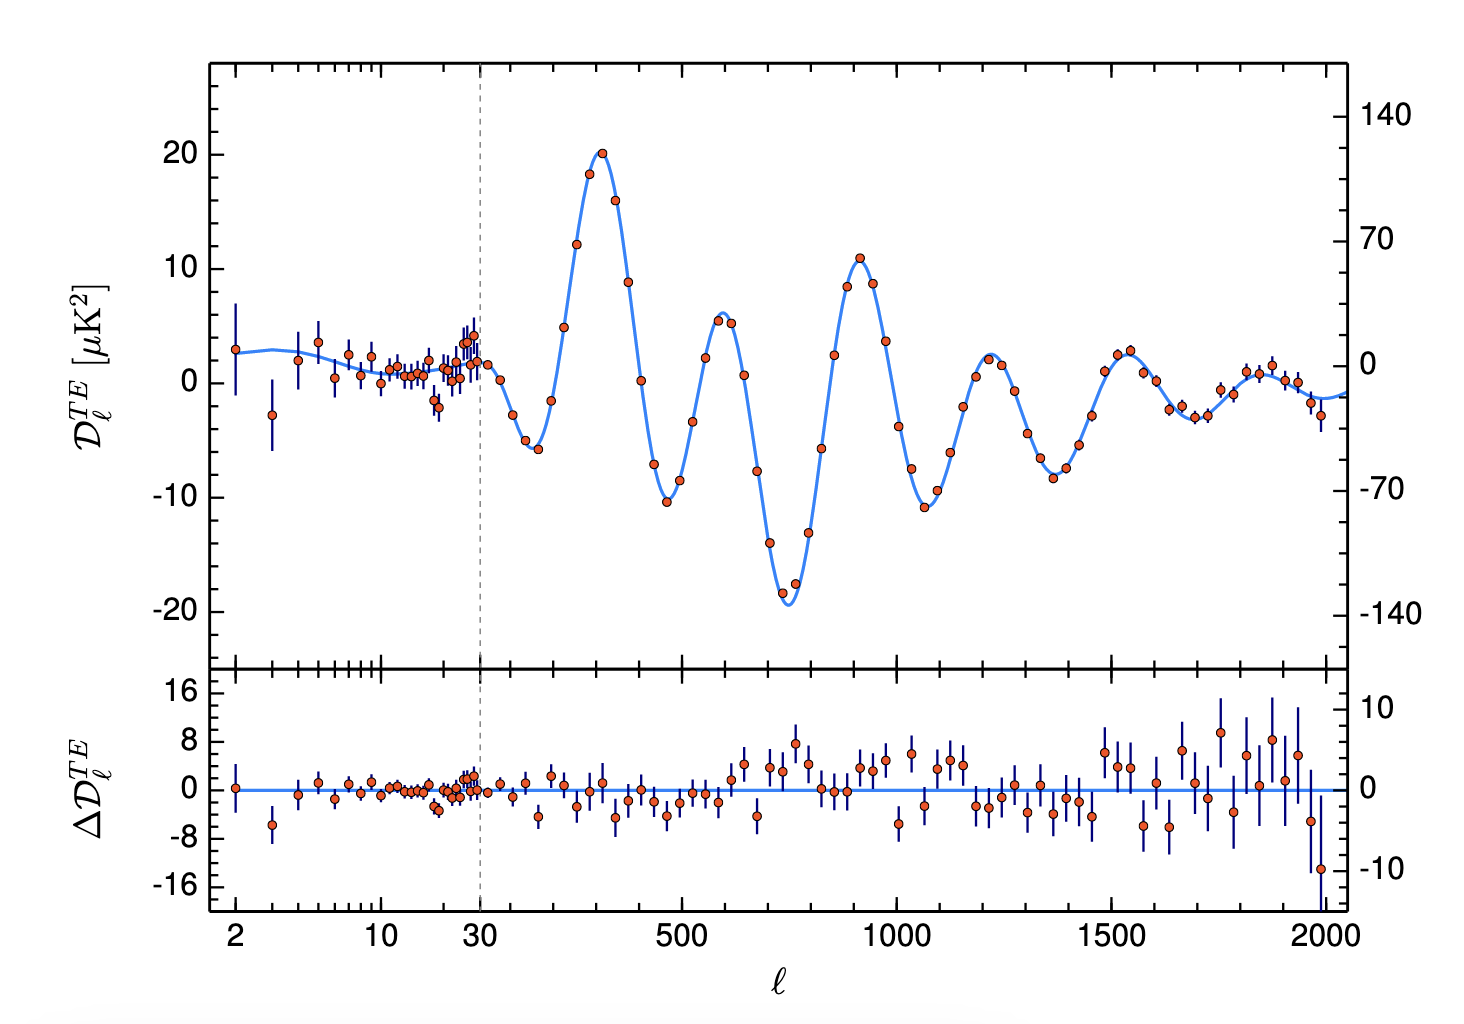
\includegraphics[width=12cm]{plots/planck_TE.png}
    \caption{Planck TE power spectrum}
    \label{fig:planck_te}
\end{figure}
\begin{figure}
    \centering
    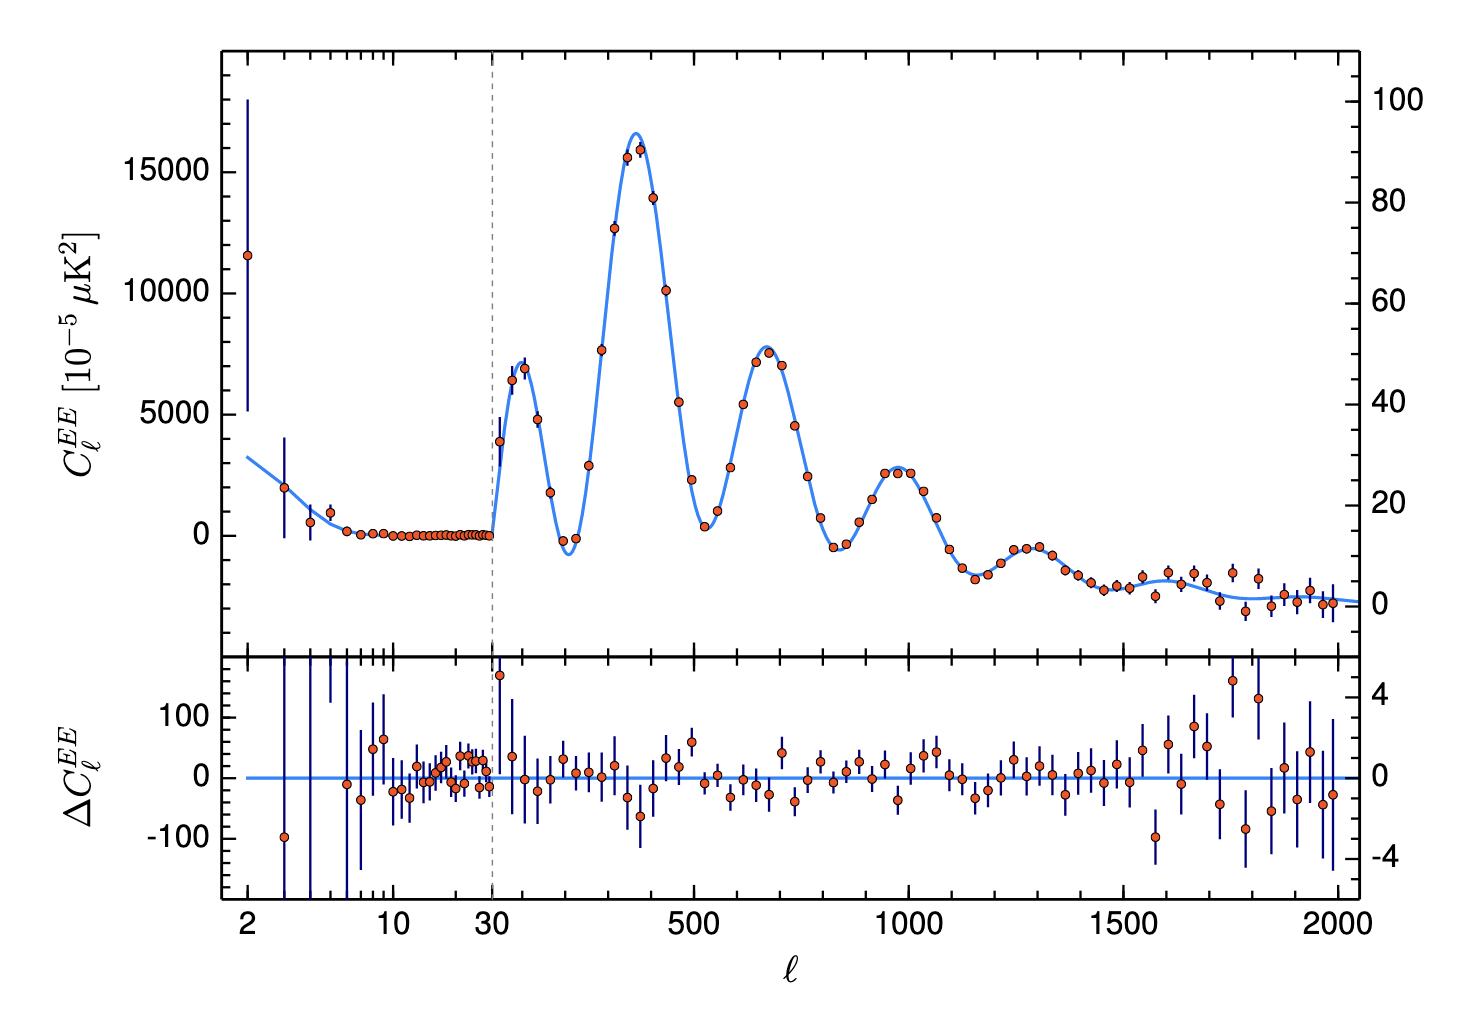
\includegraphics[width=12cm]{plots/planck_EE.png}
    \caption{Planck EE power spectrum}
    \label{fig:planck_ee}
\end{figure}
The other two power spectra are shown in figures~\ref{fig:planck_te} and~\ref{fig:planck_ee}. The main consideration with these two power spectra is to observe the way it breaks the degeneracy between $\tau_\mathrm{rei}$ and $\mathcal{A}_s,n_s$. In the TT case,  $\tau_{\mathrm{rei}}$ suppreses the power spectrum as it suppreses the fraction of light that reaches an observer. Howver, the additional scattering actual causes anisotropies in the polarization power spectrum to increase. Thus the effects of $\mathcal{A}_s$ and $\tau_\mathrm{rei}$ are similar in the TT power spectrum but opposite in the $EE$ power spectrum. Thus, one needs all 3 power spectra to reliably infer the cosmological parameters.
\section{Tensions Between Weak Lensing and CMB}
As seen, there are a total of five parameters needed to describe $\Lambda$CDM in weak lensing: $\Omega_m$, $\Omega_b$, $H_0$, $\mathcal{A}_s$, and $n_s$. This parameterization is not unique. Another common parameter, which tracks $\mathcal{A_s}$, is $\sigma_8$
\begin{equation}
	\sigma_8^2 = \left.\int\limits_0^\infty P(k,r)\left(\frac{3j_1(kr)}{kr}\right)^2\frac{k^2}{2\pi^2}dk\right|_{r=8}
\end{equation}
which can be described as the amplitude of matter fluctuations at the scale $8 h^{-1}\mathrm{Mpc}$. With this parameter instead of $\mathcal{A}_s$, weak lensing gives string constraints on $S_8 = \sigma_8\sqrt{\Omega_m/0.3}$. 

The reality is, however, that CMB measurements of some of these parameters differ between the parameters measured from weak lensing (precise results can be found in~\cite{amon_dark_2022,noauthor_planck_2018}). The most famous discrepancy is the $H_0$ tension (figure~\ref{fig:h0_tension}). Weak lensing measurements are significantly higher than CMB measurements; a nearly $5\sigma$ difference. The other famous tension is the $S_8$ tension at about a $3\sigma$ difference (figure~\ref{fig:s8_tension}). There have been extensive efforts to propose a model that can resolve these tensions (modified gravity, early dark energy, quintessence, etc.), but as of now no model is able to simultaneously resolve both tensions. For example, early dark energy resolves the $H_0$ tension, but the $S_8$ tension tends to either remain the szme or increase. The remaining chapters will explore how to compute these tensions and demonstrate a proposed consistency test.
\begin{figure}[ht]
	\centering
	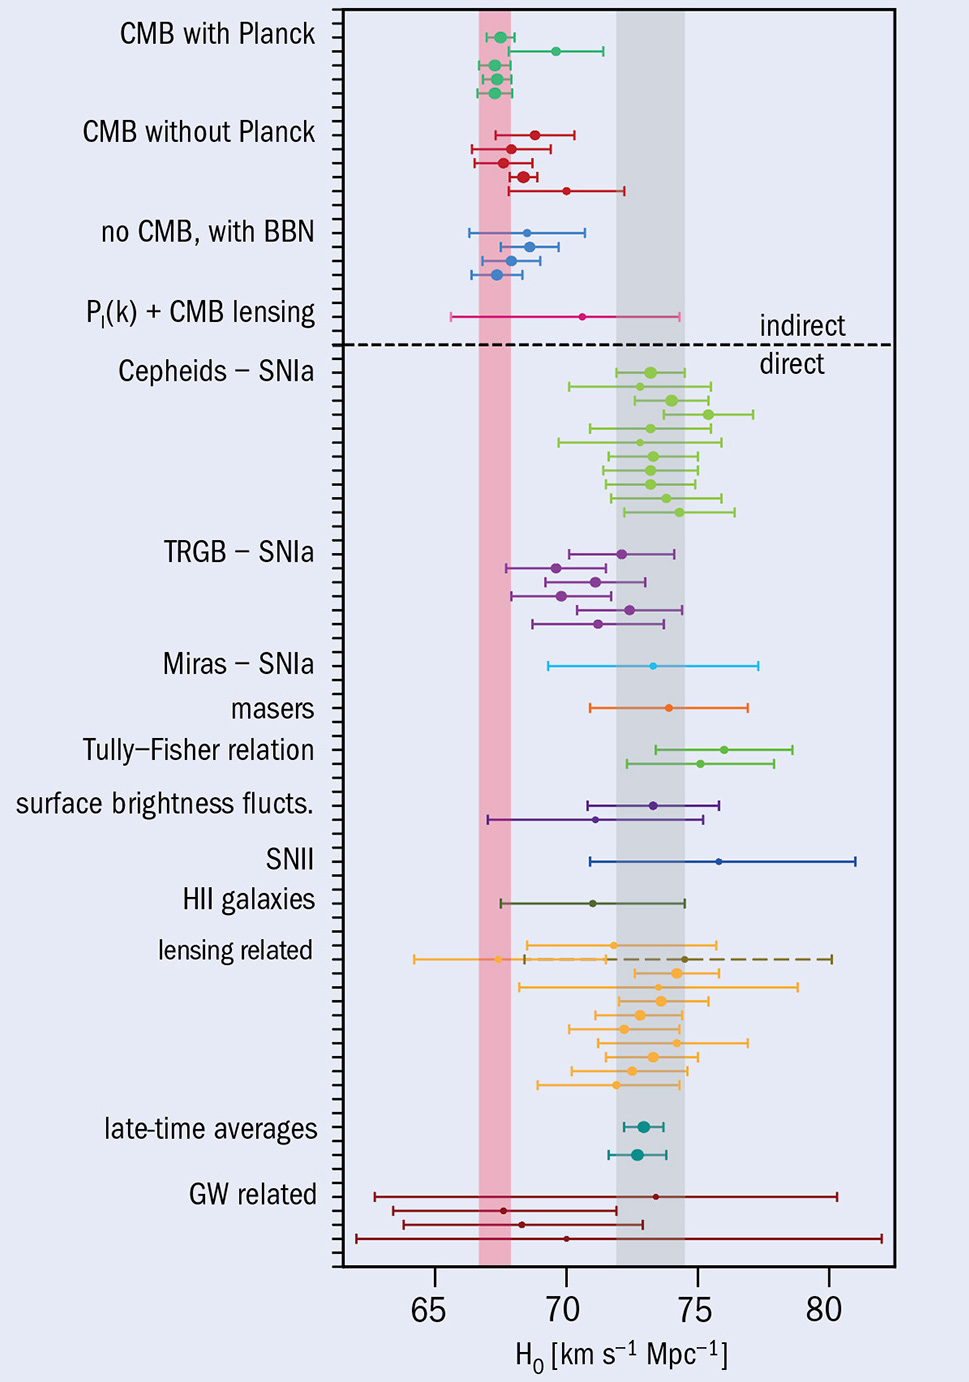
\includegraphics[width=0.75\textwidth]{plots/h0_tension.jpg}
	\caption{Measurements of $H_0$ from different experiements.}
	\label{fig:h0_tension}
\end{figure}
\begin{figure}[ht]
	\centering
	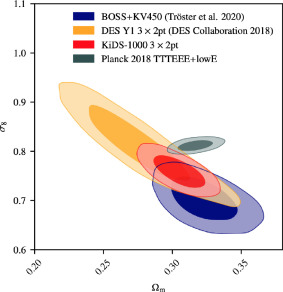
\includegraphics[width=0.75\textwidth]{plots/s8_tension.jpg}
	\caption{Measurements of $S_8$ from different experiements.}
	\label{fig:s8_tension}
\end{figure}








